% Definition of radii
\def\firstradius{(0,0) circle (1.5cm)}
\def\firstnode{(0,0) circle (0.1cm)}

\def\secondradius{(1,0) circle (1.5cm)}
\def\secondnode{(1,0) circle (0.1cm)}

\def\thirdradius{(2,0) circle (1.5cm)}
\def\thirdnode{(2,0) circle (0.1cm)}

\colorlet{circle edge}{black!100}
\colorlet{circle area}{gray!20}

\tikzset{
  filled/.style={fill=circle area, draw=circle edge, thick},
  outline/.style={draw=circle edge, thick},
  strong/.style={draw=circle edge, ultra thick},
  dash/.style={very thick, dashed}
}

\setlength{\parskip}{5mm}
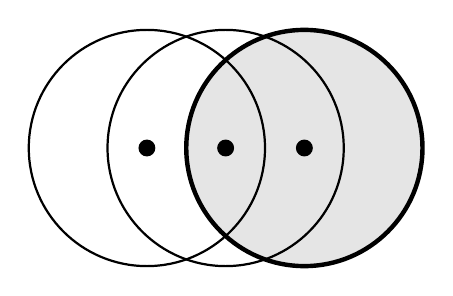
\begin{tikzpicture}
  \begin{scope}
    \fill[filled] \thirdradius;
  \end{scope}

  \fill[black] \firstnode;
  \fill[black] \secondnode;
  \fill[black] \thirdnode;

  \draw[outline] \firstradius node {};
  \draw[outline] \secondradius node {};
  \draw[strong] \thirdradius node {};

  \draw \firstnode node {};
  \draw \secondnode node {};
  \draw \thirdnode node {};
\end{tikzpicture}
